\documentclass[conference]{IEEEtran}
\IEEEoverridecommandlockouts
\usepackage{cite}
\usepackage{amsmath,amssymb,amsfonts}
\usepackage{graphicx}
\usepackage{textcomp}
\usepackage{xcolor}
\usepackage{booktabs}

\def\BibTeX{{\rm B\kern-.05em{\sc i\kern-.025em b}\kern-.08em
    T\kern-.1667em\lower.7ex\hbox{E}\kern-.125emX}}

% Convenience macro for sections that are intentionally left as
% headings only, pending implementation. Remove/replace as each
% component is built.
\newcommand{\pending}{\textit{[Section pending -- to be completed once this component is implemented.]}}

\begin{document}

\title{An Autonomous Aerial Surveillance and Digital Twin Framework for Traffic Violation Detection and Road Surface Anomaly Monitoring\\
\large \textit{(Working Draft)}}

\author{
\IEEEauthorblockN{1\textsuperscript{st} Afif Showfeer}
\IEEEauthorblockA{
\textit{Dept. of ---} \\
\textit{--- Institution} \\
City, Country \\
email@placeholder.edu}
}

\maketitle

\begin{abstract}
Urban road networks are monitored today through fixed-point CCTV and periodic manual inspection, leaving most of the network unobserved between fixed installations and leaving road-surface condition tracked only reactively, after complaints or accidents. This paper presents an autonomous aerial surveillance framework that uses unmanned aerial vehicle (UAV) footage, computer-vision detection and tracking, and a planned three-dimensional digital twin to give traffic authorities and city planners continuous, spatially structured visibility into both traffic behaviour and road surface condition. \textbf{The central claim of this work is not enforcement -- the system is not designed to cite, fine, or dispatch officers against individual drivers. Its purpose is simulation-driven decision support: detected vehicle behaviour and road-surface conditions are replayed and projected inside a shared digital twin so that a proposed intervention -- a new signal, a lane reconfiguration, a resurfacing priority, a one-way conversion -- can be simulated and evaluated for effectiveness before it is committed to in the real world.} An early exploratory draft of the project briefly included enforcement-adjacent mechanisms (automatic number-plate recognition and challan generation); these were never the project's core thesis and were dropped once the scope was clarified around simulation and planning support rather than citation issuance. This paper reports the parts of the framework that are implemented and empirically evaluated to date: a YOLO26l vehicle detector fine-tuned on the VisDrone2019-DET aerial dataset (overall mAP@50 = 0.457, car class mAP@50 = 0.832, $\approx$85 FPS on an RTX 4060 Laptop GPU), a ByteTrack-based multi-object tracker validated for identity stability on real drone footage, a YOLO26l-seg instance-segmentation baseline for pothole detection trained on the PothRGBD dataset (box mAP@50 = 0.923, mask mAP@50 = 0.927), a per-frame vehicle trajectory extraction pipeline, and a CARLA+AirSim synthetic-aerial-footage simulation pipeline with a confirmed working capture-detect-track loop. The remaining architecture defined in the project's Product Requirements Document -- the violation rule engine, pixel-to-GPS geo-projection, the CesiumJS-based digital twin, the FastAPI/PostGIS/Redis backend, the DBSCAN-based urban planning recommendation engine, the automated reporting layer, and the role-based dashboards -- is presented here as designed system architecture with its implementation status explicitly marked as pending, to be completed and evaluated in subsequent work.
\end{abstract}

\begin{IEEEkeywords}
UAV surveillance, digital twin, object detection, YOLO, multi-object tracking, ByteTrack, road surface anomaly detection, pothole segmentation, urban planning, CARLA simulation, aerial imagery
\end{IEEEkeywords}

\section{Introduction}

Cities generate a continuous stream of traffic and road-infrastructure problems -- unsafe driving behaviour, deteriorating road surfaces, and emerging congestion patterns -- that existing monitoring infrastructure is not built to observe systematically. Ground-level CCTV and automatic number-plate recognition (ANPR) installations cover fixed points, not continuous areas: they suffer from fixed fields of view, occlusion from buildings and other vehicles, single-plane perspective with no trajectory information, and no cross-zone awareness. Road surface degradation -- potholes, cracking, waterlogging, and debris -- is typically identified only reactively, through citizen complaints, vehicle-damage claims, or accidents, rather than through a continuously updated, geo-tagged condition inventory. City planners, in turn, are left to make infrastructure decisions from anecdotal complaint data and periodic manual surveys rather than continuous, structured evidence, and have no way to test a proposed change -- a new signal, a lane reconfiguration, a one-way conversion -- before committing budget to it.

This project proposes an aerial surveillance framework, built around UAV-captured video, to address this gap. Detected vehicles and road-surface defects are converted into structured, geo-tagged events that feed a shared three-dimensional digital twin of the monitored road network. The twin is not a passive map: it is a simulation environment in which a planner can construct a proposed change -- add a signal, close a lane, convert a road to one-way, reprioritize a resurfacing schedule -- and have the system project that change's effect against the historical event data already collected, so that what actually works can be identified before any physical or administrative action is taken.

\subsection{Positioning: Simulation-Driven Decision Support, Not Law Enforcement}

It is important to state explicitly what this system is and is not, since aerial vehicle detection is frequently associated with enforcement. \textbf{The system's core claim is a simulation and decision-support capability, not a citation or enforcement pipeline.} Detected traffic behaviour and road-surface condition exist, in this framework, to populate a digital twin that can be run forward under a hypothetical intervention -- this is closer to a planning flight-simulator for road infrastructure than to an automated ticketing system. An early exploratory draft of the project's requirements briefly specified enforcement-adjacent mechanisms -- automatic number-plate recognition (ANPR) triggering, automatic legal challan generation, and officer dispatch -- inherited from a more conventional "traffic violation detection" framing. These were never the project's actual thesis and have since been dropped from scope entirely: no component described in this paper identifies, cites, or reports individual drivers or vehicles to any authority. The system's outputs are aggregate, spatial, and intended for infrastructure and policy decisions, not individual-level enforcement action.

\subsection{Contributions}

This paper makes the following contributions:
\begin{itemize}
    \item An aerial vehicle detector (YOLO26l) fine-tuned and evaluated on the VisDrone2019-DET dataset, reported with full per-class metrics.
    \item A ByteTrack-based multi-object tracking layer validated for identity stability on real UAV footage.
    \item A road-surface anomaly (pothole) segmentation baseline (YOLO26l-seg) trained and evaluated on the PothRGBD dataset.
    \item A working CARLA+AirSim synthetic aerial data-capture and validation pipeline.
    \item A complete system architecture -- spanning violation detection, digital twin visualization, geo-spatial mapping, backend infrastructure, urban planning recommendation, and automated reporting -- presented as designed but not yet implemented, to scope the remaining work explicitly.
\end{itemize}

\subsection{Paper Organization}

Section II reviews related work. Section III presents the overall system architecture and objective-by-objective implementation status. Section IV describes the methodology and configuration of each implemented component. Section V reports quantitative results. Section VI outlines each planned-but-not-yet-implemented component as scoped by the system architecture. Section VII discusses current limitations, and Section VIII concludes with a roadmap for remaining work.

\section{Related Work}

\subsection{Digital Twins in Urban Planning}

City-scale digital twins are an established and rapidly growing practice in urban planning: municipal and commercial platforms already build synchronized virtual replicas of cities from IoT, traffic, and sensor feeds to let planners run what-if scenarios -- a new transit line, a zoning change, a storm event -- and observe projected effects before committing resources~\cite{gravel2gavel,cityplanner}. Market analyses place this as a multi-billion-dollar and growing segment of smart-city infrastructure spending~\cite{kgt2026}. This confirms that the general concept of a simulation-capable digital twin for city planning is not novel in itself; it is an active, deployed practice.

\subsection{UAV-Based Digital Twins for Roads and Traffic}

Closer to this project's specific combination, recent research has begun connecting UAVs, computer vision, and digital twins for road-network monitoring. Traffic-aware digital twin simulators have been proposed specifically for UAV-based pavement inspection, providing configurable virtual road networks to test detection and flight strategies before real deployment~\cite{uavpavement}. Drone-derived vehicle trajectory datasets such as CitySim have been built explicitly to support digital-twin-based traffic safety research~\cite{citysim}, and digital twins that couple microscopic traffic simulation with vehicle dynamics have been used for traffic safety analysis using surrogate safety measures~\cite{trafficsafetytwin}.

\subsection{Gap Addressed by This Work}

To the best of our knowledge, no existing published system combines, in one pipeline: (i) UAV aerial vehicle-behaviour detection and tracking, (ii) UAV aerial road-surface anomaly detection, (iii) a shared digital twin serving both event streams, and (iv) a spatial-clustering-driven what-if simulator that evaluates candidate infrastructure interventions against both violation and pavement-condition history. Existing digital twin platforms for urban planning are largely built on stationary sensor and administrative data rather than continuous aerial computer vision~\cite{gravel2gavel,kgt2026}; existing UAV-digital-twin research to date targets either pavement inspection~\cite{uavpavement} or vehicle trajectory/safety analysis~\cite{citysim,trafficsafetytwin} in isolation, not both jointly feeding one planning-oriented twin. This is the specific gap this project's architecture (Section III) is designed to address; as noted throughout this paper, most of that architecture remains to be implemented and evaluated.

\section{System Architecture and Implementation Status}

The proposed framework is organized into five integrated pillars, per the project's Product Requirements Document (v2.0): (1) an Aerial Detection Engine for vehicle detection and tracking, (2) a Road Surface Anomaly Engine for pavement defect detection, (3) a Digital Twin Environment for shared 3D visualization and scenario simulation, (4) an Automated Analysis and Reporting Layer, and (5) an Intelligent Urban Planning Engine. Architecturally, the system is layered as: an \textit{input layer} (CARLA simulator frames or real UAV RTSP/telemetry), a \textit{detection pipeline layer} (parallel vehicle and road-surface computer-vision models sharing a geo-projection engine), a \textit{violation and anomaly engine layer} (rule evaluation and severity scoring), a \textit{backend infrastructure layer} (API, persistent geo-spatial storage, live state, object storage), an \textit{analysis, reporting and planning layer} (spatial clustering, recommendation generation, report compilation), and a \textit{presentation layer} (role-based dashboards embedding the shared digital twin).

Table~\ref{tab:status} summarizes the implementation status of each primary project objective at the time of writing.

\begin{table}[htbp]
\caption{Implementation status by project objective}
\label{tab:status}
\centering
\begin{tabular}{@{}p{0.09\linewidth}p{0.58\linewidth}p{0.23\linewidth}@{}}
\toprule
\textbf{Obj.} & \textbf{Description} & \textbf{Status} \\
\midrule
1 & Traffic violation detection (vehicle detection + tracking + 10 violation types) & Detection \& tracking implemented; violation rule engine not yet implemented \\
2 & Digital twin (CesiumJS 3D visualization) & Not implemented \\
3 & Road surface anomaly detection (pothole, crack, waterlogging, debris) & Pothole segmentation baseline implemented; other three classes not implemented \\
4 & Intelligent urban planning \& recommendation engine (DBSCAN + what-if simulator) & Not implemented \\
5 & Automated analysis and reporting layer & Not implemented \\
6 & Improved road safety / infrastructure outcomes (end-to-end traceability) & Dependent on Objectives 1--5; not yet achievable \\
7 & Geo-spatial pixel-to-GPS coordinate mapping & Not implemented \\
8 & CARLA-based simulation and validation & Capture/detect/track pipeline implemented; quantitative validation run pending \\
9 & Scalable backend infrastructure (FastAPI, PostgreSQL/PostGIS, Redis, MinIO) & Not implemented \\
\bottomrule
\end{tabular}
\end{table}

\section{Implemented Components: Methodology}

\subsection{Aerial Vehicle Detection}

The vehicle detection model is YOLO26l (Ultralytics), fine-tuned on the VisDrone2019-DET dataset (6{,}471 training images, 548 validation images), using axis-aligned bounding boxes across the dataset's native classes (car, van, truck, bus, motor, pedestrian, people, bicycle, tricycle, awning-tricycle). An oriented bounding box (OBB) variant on the DOTA dataset was evaluated and deliberately not carried forward, since downstream tracking datasets (VisDrone-MOT, UAVDT) provide only axis-aligned annotations. Training was run for up to 300 epochs with a 10-hour wall-clock cap and an early-stopping patience of 20 epochs, at image size 640, batch size 8, on a single RTX 4060 Laptop GPU (8~GB VRAM).

\subsection{Multi-Object Tracking}

Tracking is performed with ByteTrack, via Ultralytics' built-in \texttt{model.track()} integration, applied directly on top of the fine-tuned detector with no additional training required, since ByteTrack is a classical (non-learned) association algorithm. Tracking was restricted to the car, van, truck, and bus classes; motorcycle tracking was evaluated and excluded after it produced severe identity churn on small, frequently occluded objects, which is not relevant to the violation types currently in scope.

\subsection{Vehicle Trajectory Extraction}

A trajectory extraction stage runs the detector and tracker together over a video source and records, per frame and per track identifier, the object class, bounding-box centroid, width, height, and detection confidence, to a CSV file. This trajectory data is the intended foundation for the violation rule engine (Section VI-A) and for the geo-projection and anomaly-deduplication logic, but is not yet consumed by any downstream rule logic.

\subsection{Road Surface Anomaly Detection: Pothole Segmentation Baseline}

A stock (architecturally unmodified) YOLO26l-seg model was fine-tuned on the PothRGBD dataset (1{,}000 RGB-D images, split 800/100/100 into train/validation/test; only the RGB channels were used), as a reference baseline against which a planned architecture modification -- incorporating Dynamic Snake Convolution (DSConv)~\cite{dsconv}, the Simple Parameter-free Attention Module (SimAM)~\cite{simam}, and GELU activation, following the road-distress detection approach described in~\cite{roaddistress} -- is intended to be compared. Implementations of \texttt{DSConv}, \texttt{SimAM}, and a \texttt{C3k2WithSimAM} wrapper module exist in the codebase, but have not yet been integrated into the YOLO26l-seg backbone/neck graph or trained; this baseline therefore currently represents the unmodified reference point only.

\subsection{CARLA + AirSim Simulation Pipeline}

A synthetic aerial data pipeline was built on a combined CARLA and AirSim distribution ("CarlaAir"), used to generate nadir-view drone footage with known, ground-truth camera altitude, position, and orientation -- directly addressing the absence of real UAV telemetry in the public datasets used for Sections IV-A and IV-D. A script flies a simulated drone along an actual road lane (via CARLA's Waypoint API), sets the onboard camera to a nadir pose, and records JPEG frame sequences together with flight metadata. A second script re-runs the fine-tuned vehicle detector and tracker directly against these captured frames, independent of the simulator process, to validate the detection pipeline on synthetic aerial imagery. The first end-to-end run of this pipeline confirmed pipeline connectivity (capture, detection, tracking, and CSV export all completed without errors), but revealed a camera-pose configuration bug that produced skyline views instead of nadir views; this has since been fixed, and a clean quantitative re-run is pending.

\section{Results}

\subsection{Vehicle Detection Results}

Table~\ref{tab:vehicle} reports per-class detection metrics on the full VisDrone2019-DET validation split (548 images) after full training on the complete training split.

\begin{table}[htbp]
\caption{Vehicle detector (YOLO26l) results on VisDrone2019-DET validation split}
\label{tab:vehicle}
\centering
\begin{tabular}{@{}lcc@{}}
\toprule
\textbf{Class} & \textbf{mAP@50} & \textbf{mAP@50-95} \\
\midrule
Car & 0.832 & 0.586 \\
Bus & 0.600 & 0.438 \\
Van & 0.481 & 0.338 \\
Truck & 0.426 & 0.288 \\
Motor & 0.542 & 0.254 \\
Pedestrian & 0.540 & 0.258 \\
People & 0.416 & 0.170 \\
Bicycle & 0.220 & 0.098 \\
Tricycle & 0.333 & 0.187 \\
Awning-tricycle & 0.177 & 0.114 \\
\midrule
\textbf{All classes} & \textbf{0.457} & \textbf{0.273} \\
\bottomrule
\end{tabular}
\end{table}

Inference throughput was measured at 11.8~ms per image ($\approx$85~FPS) on an RTX 4060 Laptop GPU. Detection quality is strongest on the classes most relevant to the intended violation types (car, bus, van, truck) and weakest on small, frequently occluded classes (bicycle, awning-tricycle), consistent with known difficulty patterns on VisDrone.

\begin{figure}[htbp]
\centering
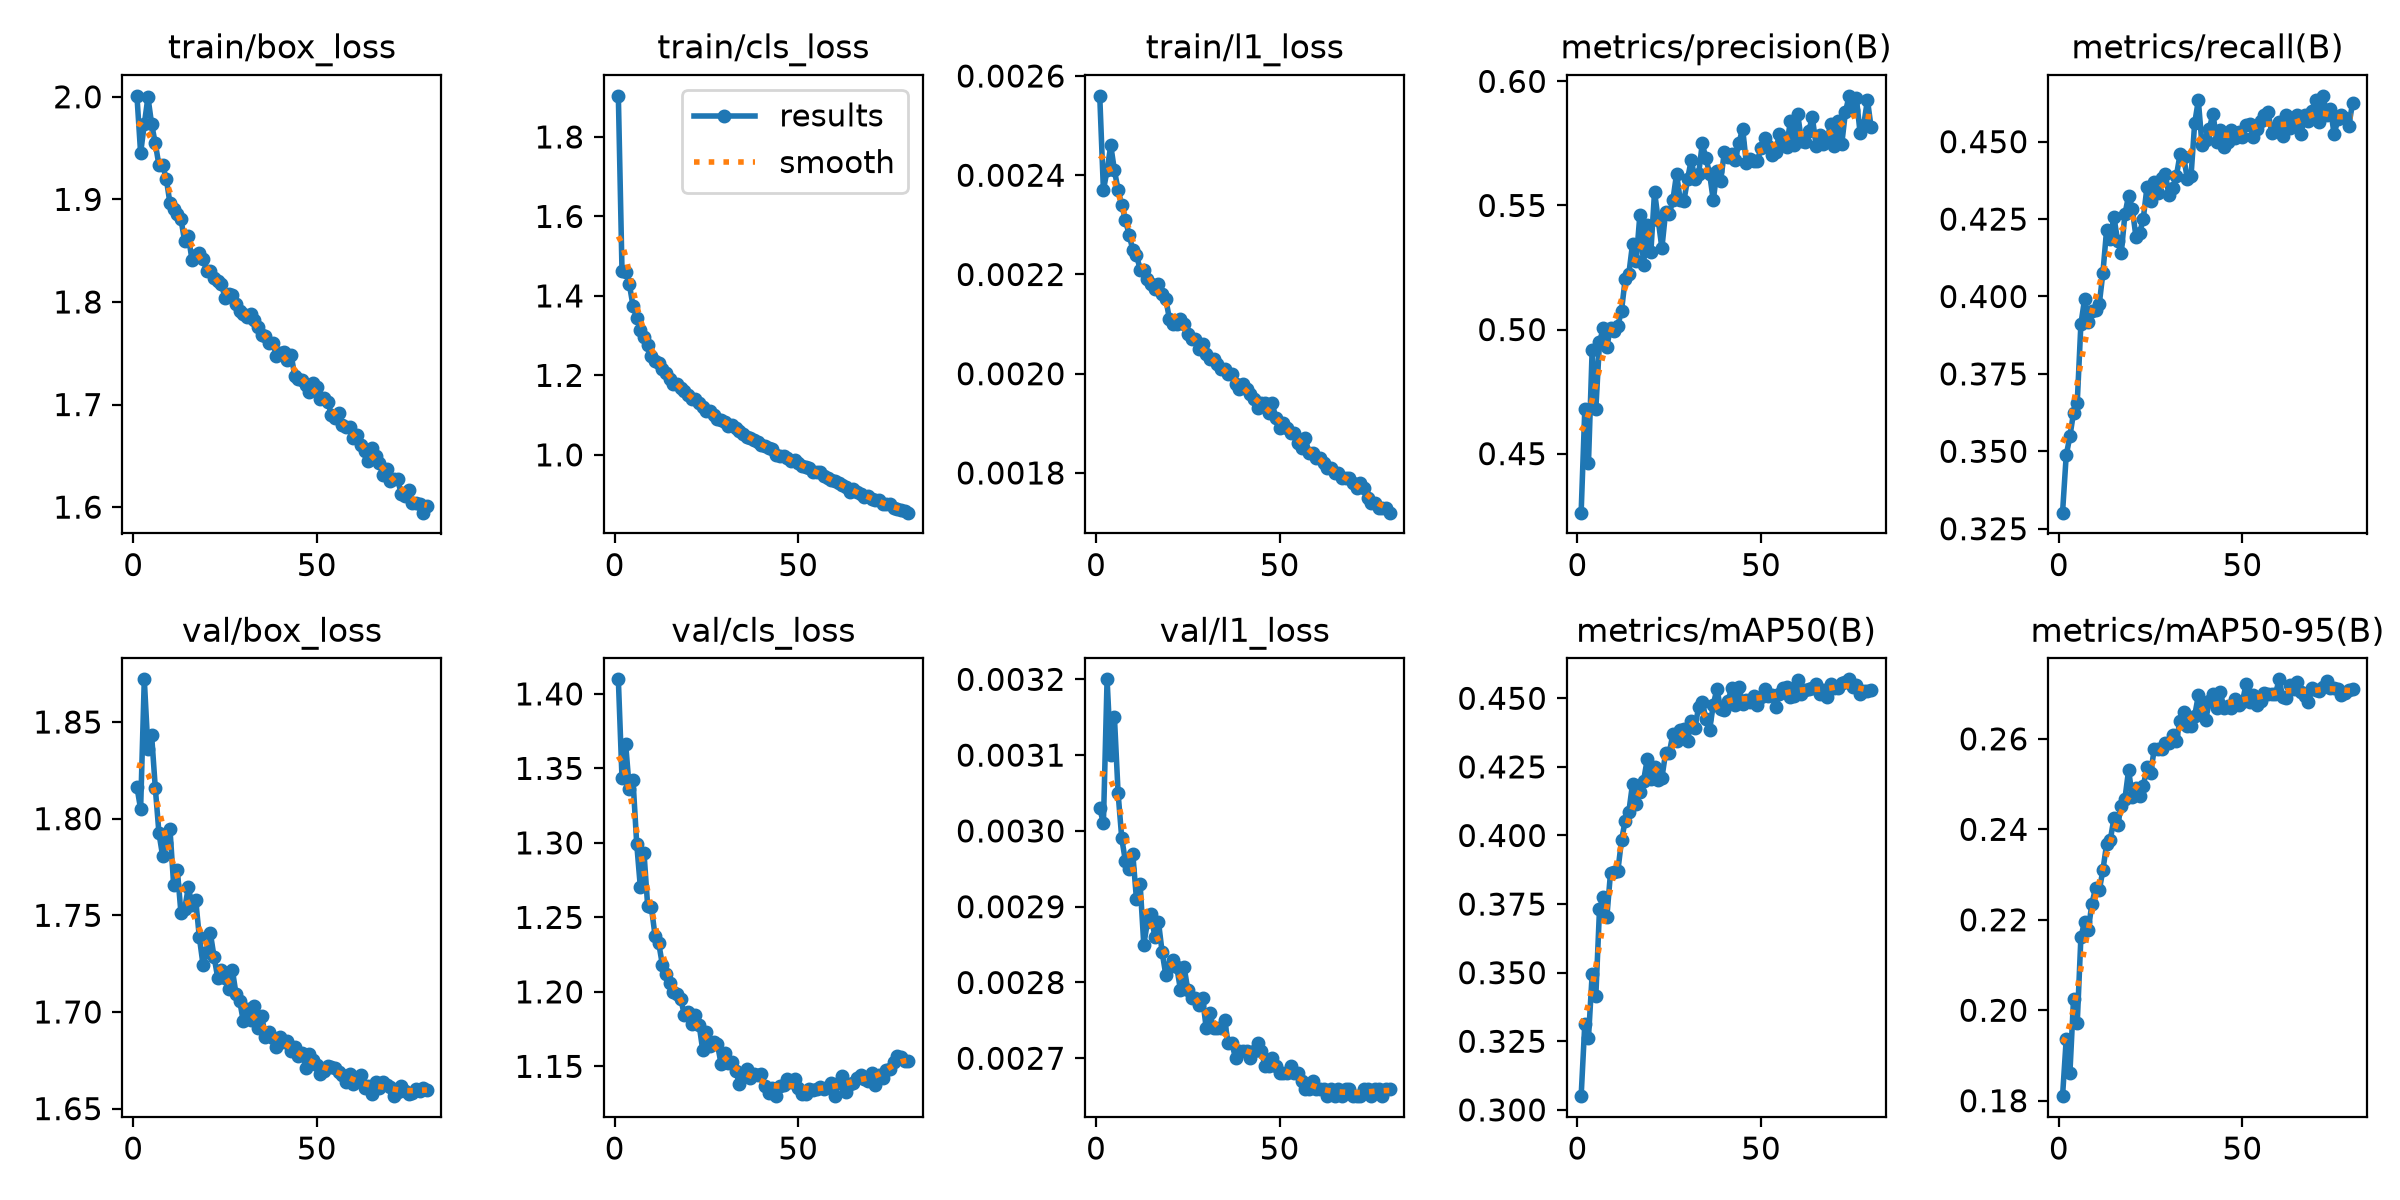
\includegraphics[width=\linewidth]{figures/vehicle_training_curves.png}
\caption{Training and validation loss/metric curves for the YOLO26l vehicle detector over the full VisDrone2019-DET fine-tuning run.}
\label{fig:veh_curves}
\end{figure}

\begin{figure}[htbp]
\centering
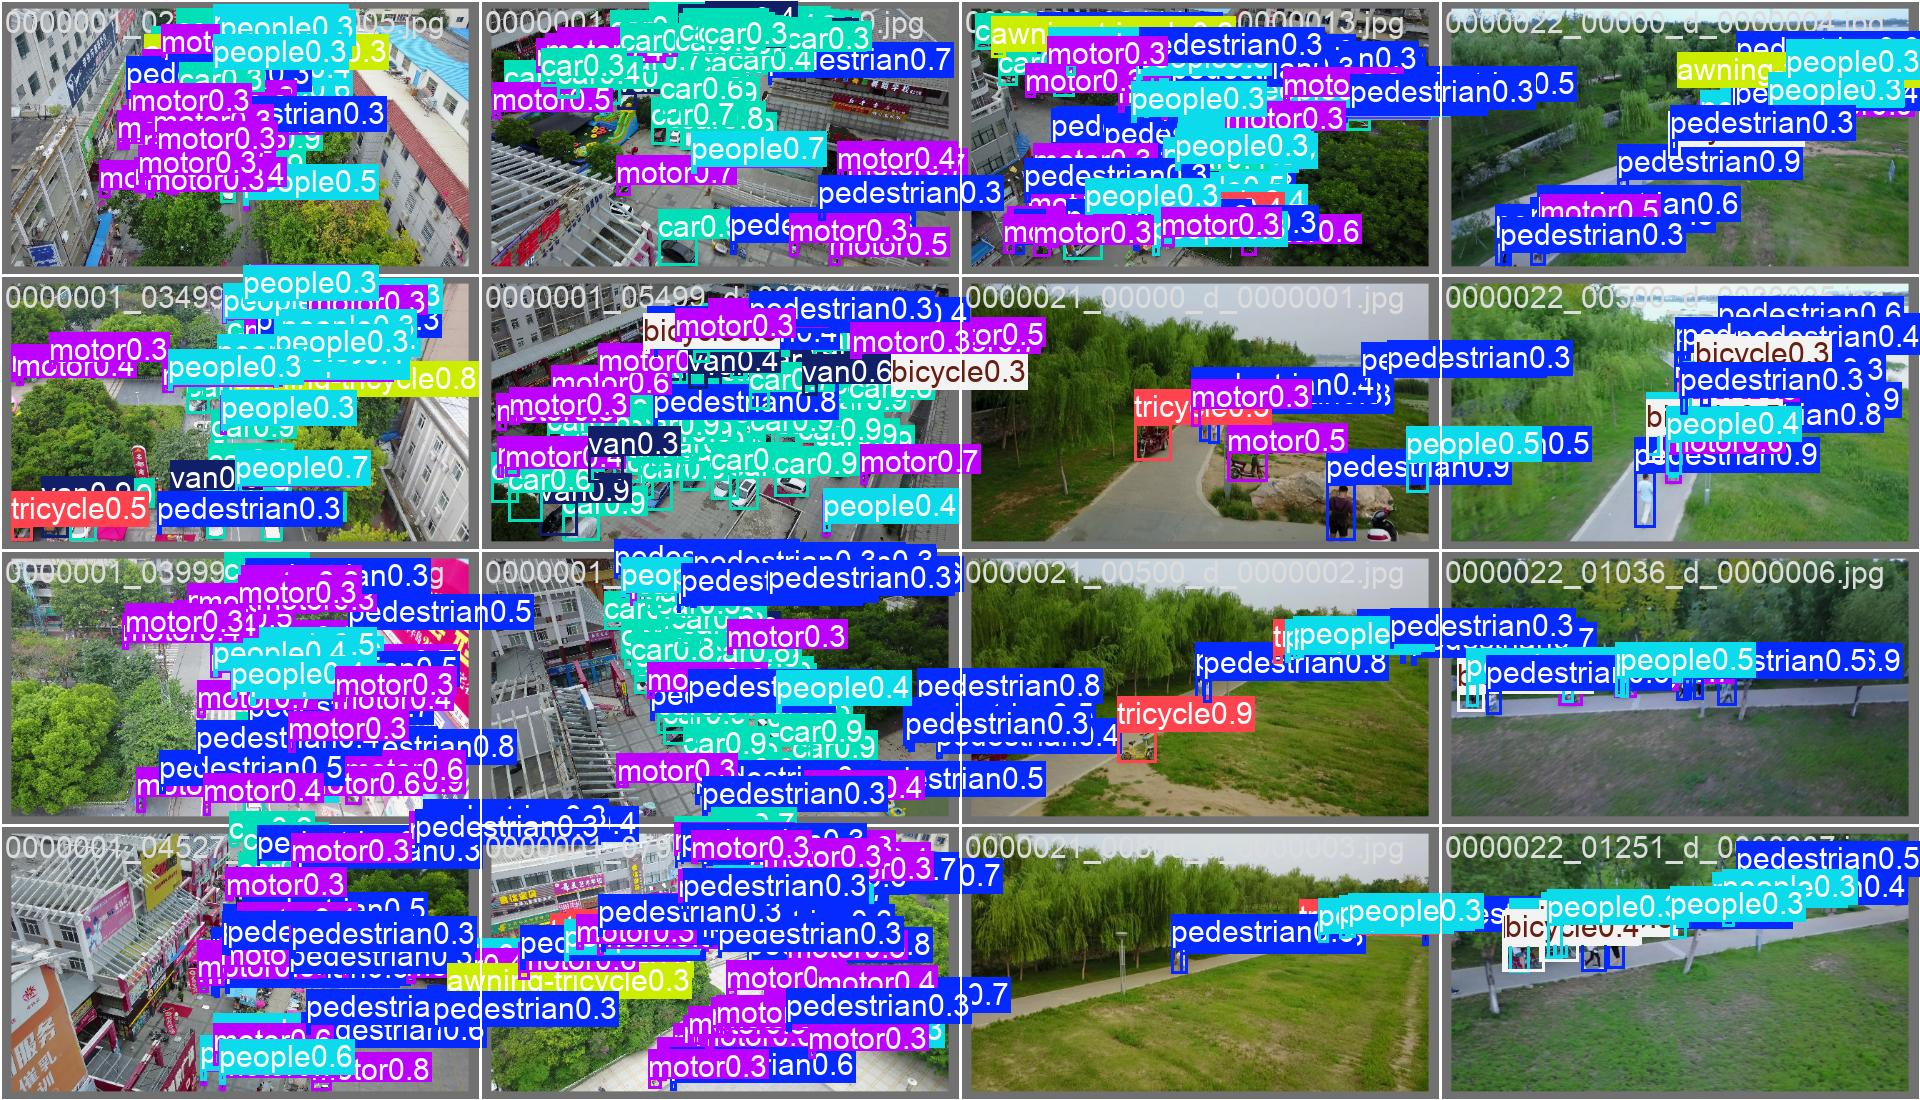
\includegraphics[width=\linewidth]{figures/vehicle_qualitative_pred.jpg}
\caption{Qualitative vehicle detections on a VisDrone2019-DET validation batch (predicted boxes and classes).}
\label{fig:veh_qual}
\end{figure}

\subsection{Multi-Object Tracking Results}

Tracking was qualitatively validated on a real, busy VisDrone2019-MOT-val intersection sequence (233 frames, sequence \texttt{uav0000137\_00458\_v}) with turning and queuing traffic plus heavy pedestrian and bicycle cross-traffic. Car, van, truck, and bus identities present from the first frame retained the same track identifier through to the final frame, with new identifiers appearing only for vehicles genuinely entering the scene later. No quantitative multi-object tracking metrics (e.g. MOTA, IDF1) have been computed to date.

\subsection{Road Surface Anomaly (Pothole) Segmentation Results}

Table~\ref{tab:pothole} reports the best-epoch validation metrics for the stock YOLO26l-seg baseline on the PothRGBD validation split, reached at epoch 51 of 71 (training stopped by early-stopping patience of 20 epochs, well inside the 10-hour time cap).

\begin{table}[htbp]
\caption{Pothole segmentation baseline (YOLO26l-seg, stock) on PothRGBD}
\label{tab:pothole}
\centering
\begin{tabular}{@{}lcc@{}}
\toprule
\textbf{Metric} & \textbf{Box} & \textbf{Mask} \\
\midrule
Precision & 0.936 & 0.956 \\
Recall & 0.838 & 0.856 \\
mAP@50 & 0.923 & 0.927 \\
mAP@50-95 & 0.605 & 0.635 \\
\bottomrule
\end{tabular}
\end{table}

This is a single-class (\textit{pothole}) result from an architecturally unmodified baseline; it is not directly comparable to the 93.7\% precision / 90.4\% recall / 93.8\% mAP@50 reported in~\cite{roaddistress}, since that work uses a different base architecture (YOLOv8) and the DSConv/SimAM/GELU modifications, neither of which has been trained here yet.

\begin{figure}[htbp]
\centering
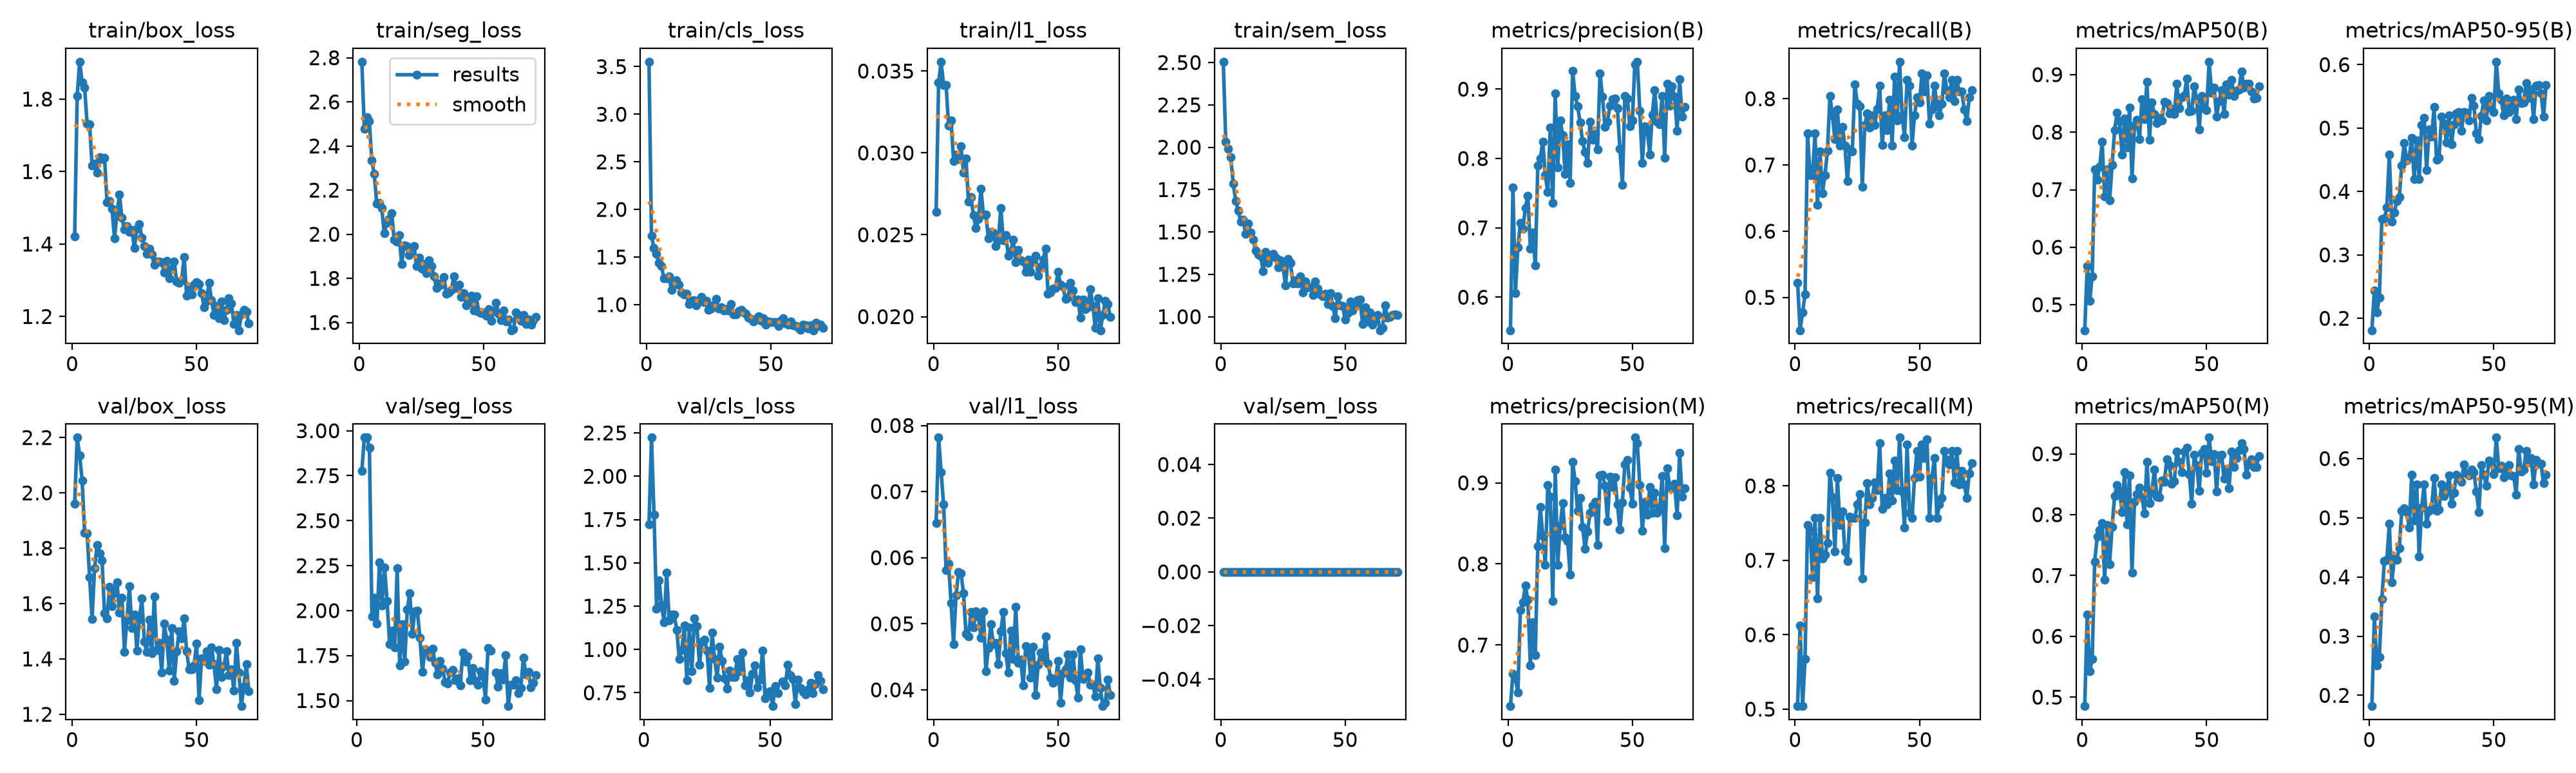
\includegraphics[width=\linewidth]{figures/pothole_training_curves.png}
\caption{Training and validation loss/metric curves for the stock YOLO26l-seg pothole segmentation baseline on PothRGBD.}
\label{fig:pot_curves}
\end{figure}

\begin{figure}[htbp]
\centering
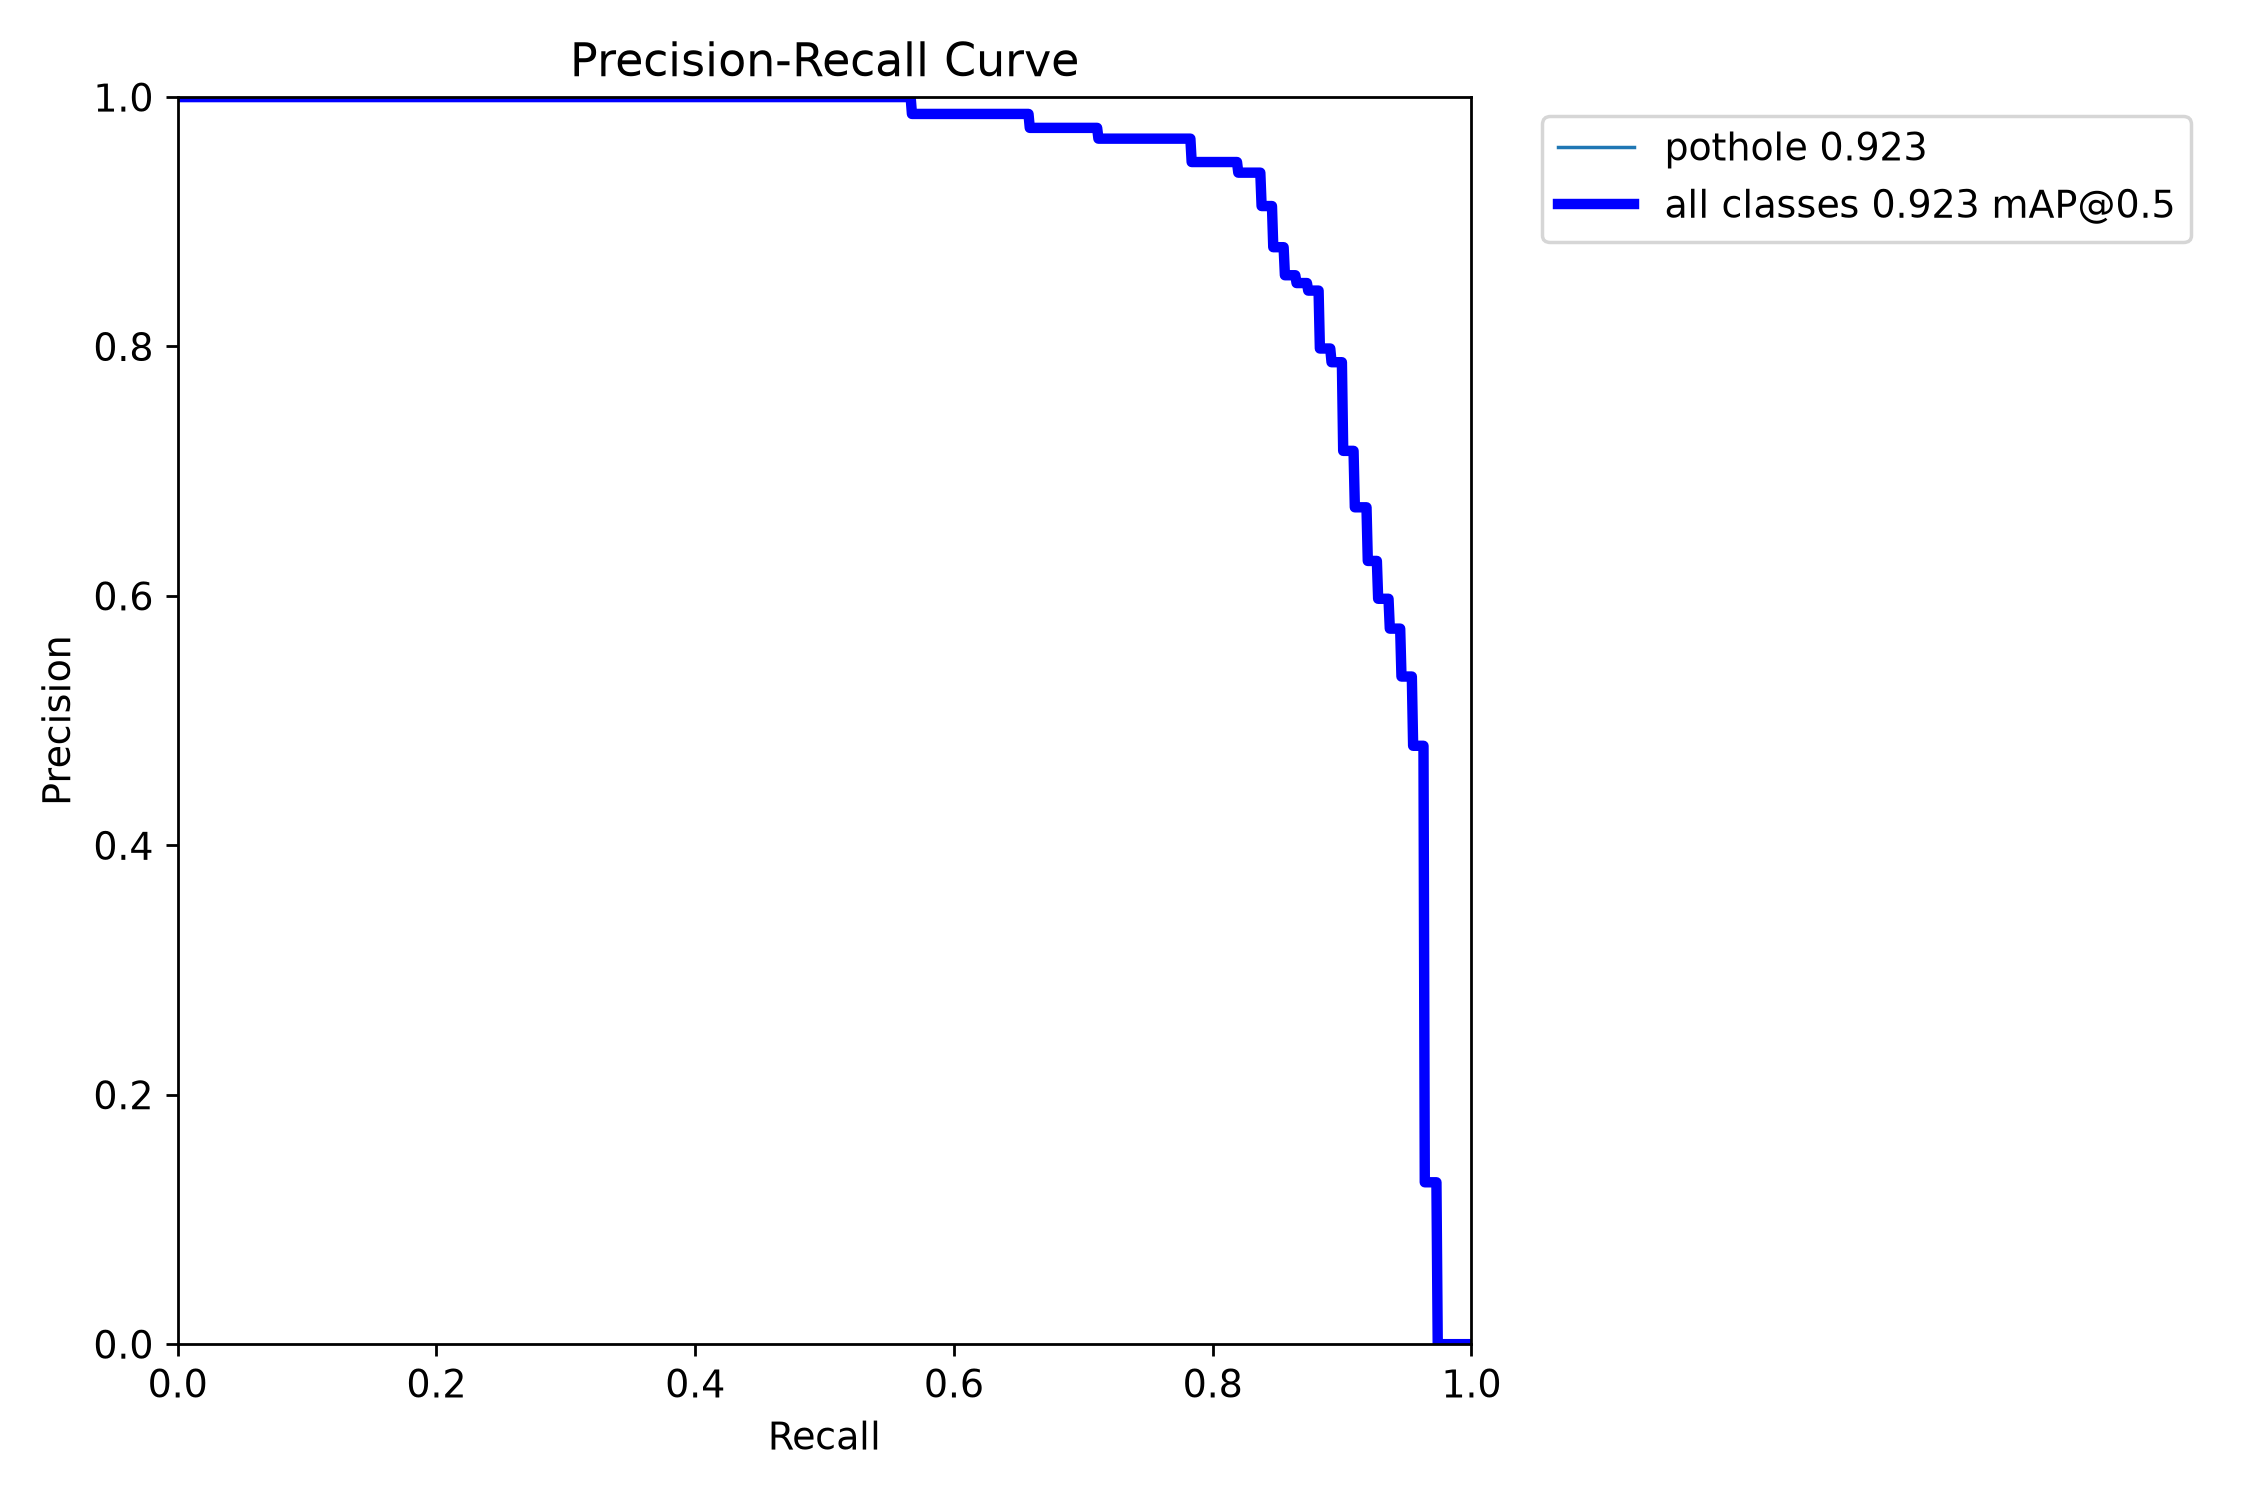
\includegraphics[width=\linewidth]{figures/pothole_pr_curve.png}
\caption{Precision--recall curve (box) for the pothole segmentation baseline on the PothRGBD validation split.}
\label{fig:pot_pr}
\end{figure}

\begin{figure}[htbp]
\centering
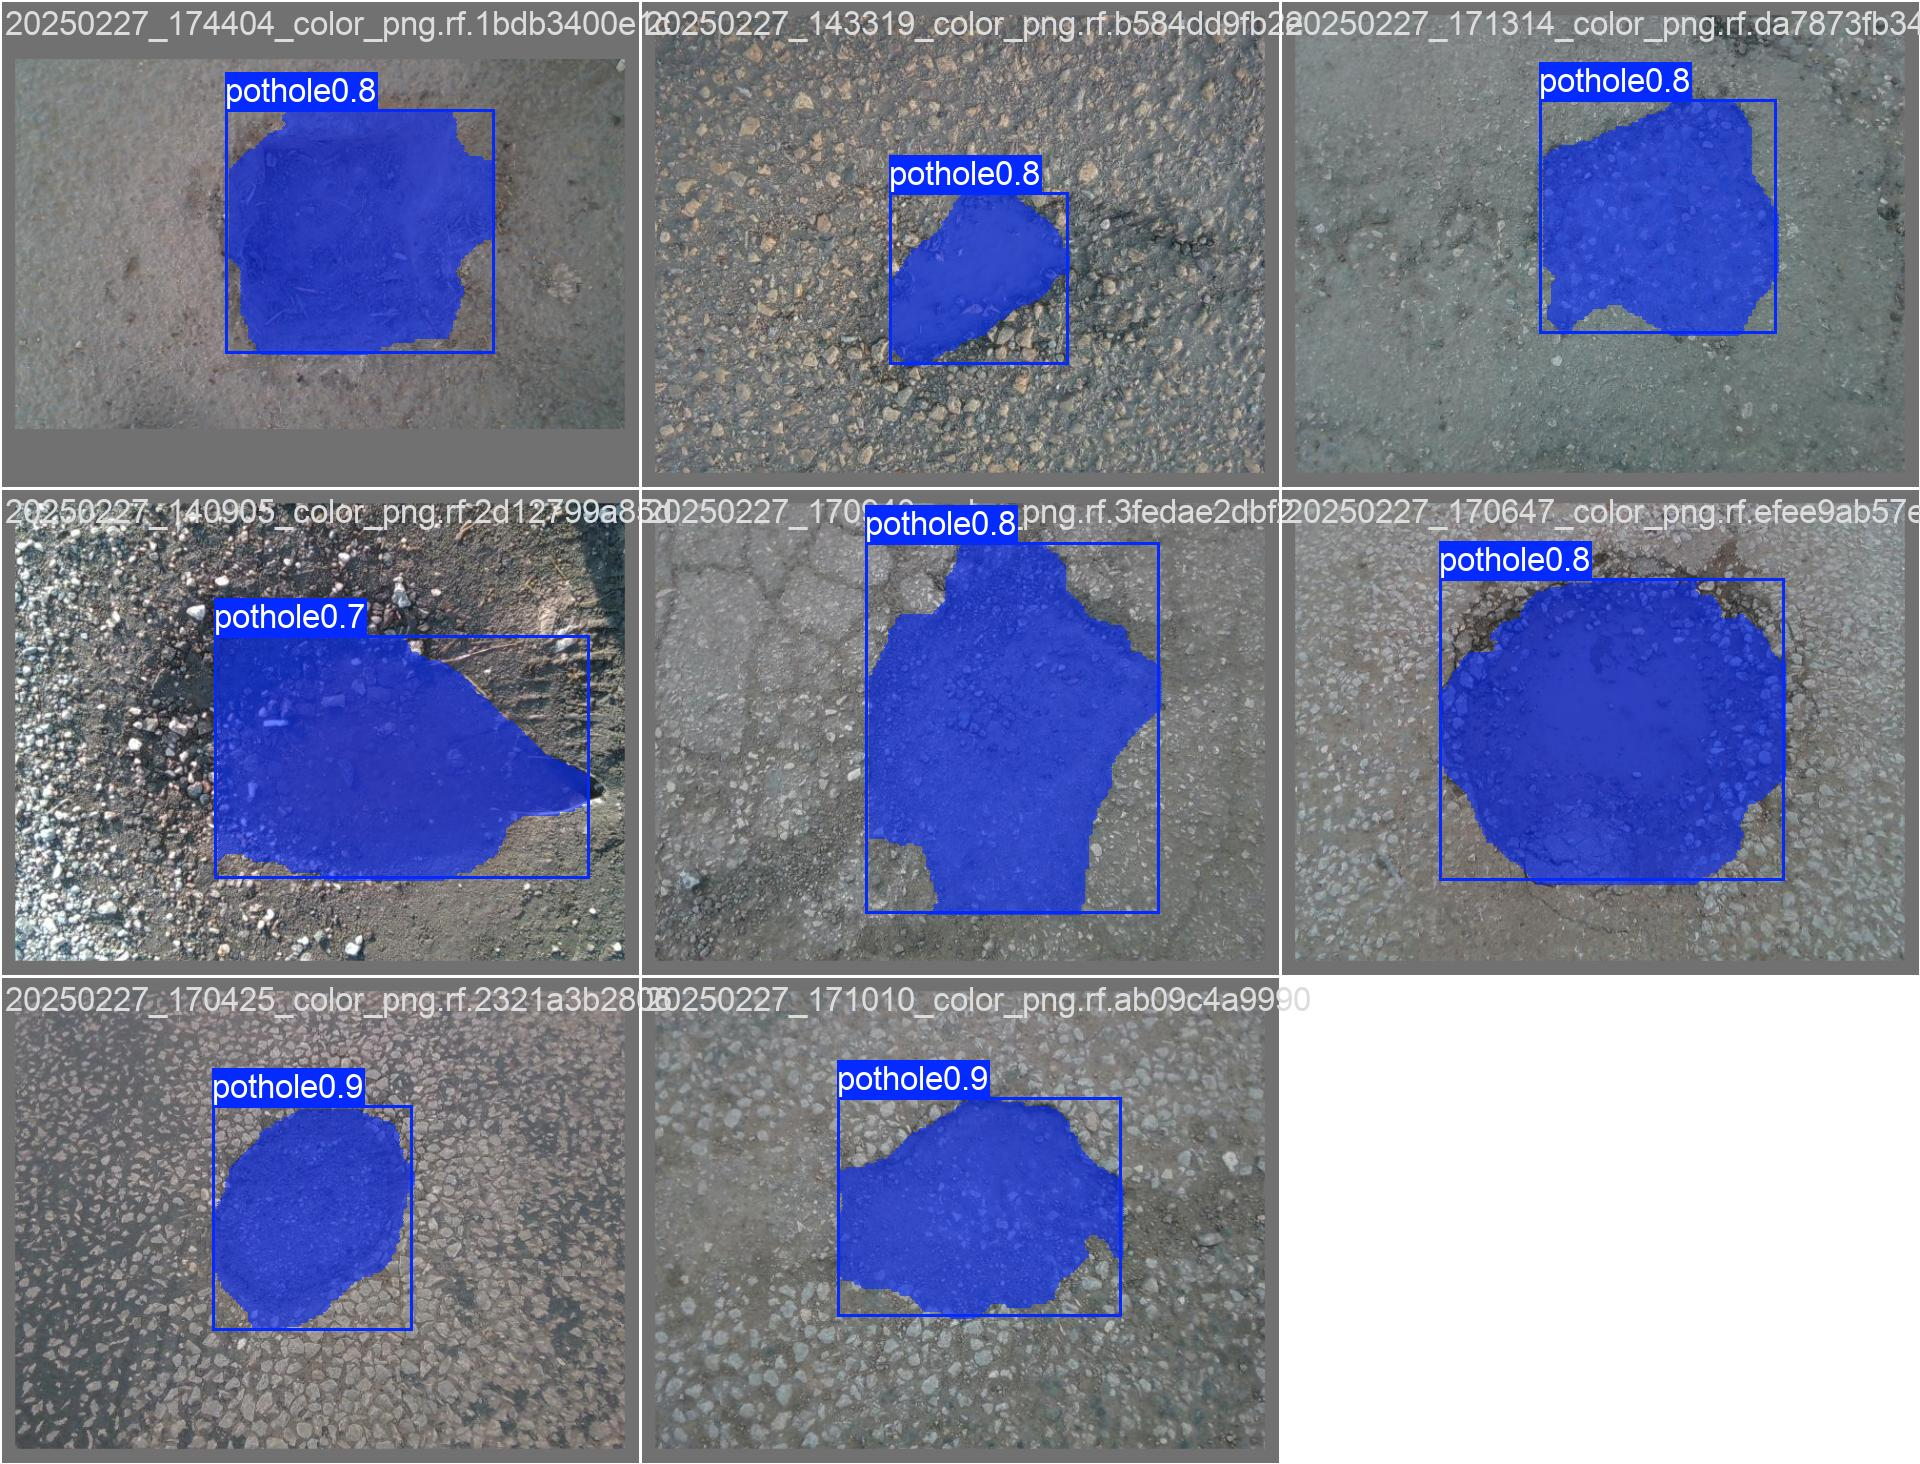
\includegraphics[width=\linewidth]{figures/pothole_qualitative_pred.jpg}
\caption{Qualitative pothole segmentation predictions on a PothRGBD validation batch.}
\label{fig:pot_qual}
\end{figure}

\subsection{Simulation Pipeline Validation}

\pending
\textit{(Quantitative detection/tracking results on CARLA+AirSim synthetic footage are pending a clean re-run following the nadir-camera configuration fix described in Section IV-E.)}

\section{Planned System Components (Not Yet Implemented)}

The following components are part of the designed system architecture (Section III) but have no implementation or evaluation to report at the time of writing. Each is retained here as a scoped heading so that the paper's structure reflects the complete intended system.

\subsection{Violation Rule Engine}
\pending

\subsection{Geo-Spatial Coordinate Mapping (Pixel-to-GPS Projection)}
\pending

\subsection{Additional Road Surface Anomaly Categories (Cracking, Waterlogging, Debris)}
\pending

\subsection{Digital Twin Visualization}
\pending

\subsection{Backend Infrastructure}
\pending

\subsection{Intelligent Urban Planning and Recommendation Engine}
\pending

\subsection{Automated Analysis and Reporting Layer}
\pending

\subsection{Role-Based Dashboards}
\pending

\section{Limitations}

The results reported in this paper are subject to several limitations. First, none of the public datasets used (VisDrone2019-DET, VisDrone2019-MOT-val, PothRGBD) include real UAV telemetry (altitude, gimbal angle, ground sample distance); the CARLA+AirSim simulation pipeline (Section IV-E) is intended to close this gap but has not yet produced a validated quantitative result. Second, the pothole segmentation baseline is trained on a relatively small dataset (1{,}000 images total) captured at ground level rather than from an aerial perspective, and its performance under a genuine aerial viewing angle and altitude has not been assessed; a domain-gap evaluation against aerial or simulated footage is planned but not yet run. Third, no violation logic has been implemented, so no claims are made in this paper about violation-detection accuracy; the reported vehicle-detection and tracking results establish only the perception layer that such logic would depend on. Fourth, tracking has been validated qualitatively only, without standard multi-object tracking metrics. Finally, the digital twin, backend, planning, and reporting layers described in Section III are architectural design only and carry no empirical validation in this paper.

\section{Conclusion and Future Work}

This paper has presented an aerial surveillance framework for traffic and road-condition monitoring that has migrated, over the course of the project, from an enforcement-centric design to a digital-twin and urban-planning-oriented governance platform. The components implemented and evaluated to date -- a fine-tuned YOLO26l vehicle detector, a ByteTrack-based tracking layer, a YOLO26l-seg pothole segmentation baseline, a trajectory extraction pipeline, and a working CARLA+AirSim synthetic data pipeline -- establish the perception layer of the proposed system. The remaining architecture, spanning the violation rule engine, geo-spatial projection, the digital twin, the backend infrastructure, the urban planning recommendation engine, and the reporting layer, is scoped and designed but remains to be implemented and evaluated. Future work will prioritize closing these gaps in roughly the order in which each depends on the last: the violation rule engine (which can be built directly on the existing trajectory extraction output), geo-spatial projection, the digital twin, the backend infrastructure, and finally the planning and reporting layers that depend on all of the above.

\section*{Acknowledgment}
\pending

\begin{thebibliography}{00}
\bibitem{ultralytics} G. Jocher, A. Chaurasia, and J. Qiu, ``Ultralytics YOLO,'' 2023. [Online]. Available: https://github.com/ultralytics/ultralytics
\bibitem{bytetrack} Y. Zhang, P. Sun, Y. Jiang, D. Yu, F. Weng, Z. Yuan, P. Luo, W. Liu, and X. Wang, ``ByteTrack: Multi-Object Tracking by Associating Every Detection Box,'' in \textit{Proc. European Conference on Computer Vision (ECCV)}, 2022.
\bibitem{visdrone} P. Zhu, L. Wen, D. Du, X. Bian, H. Fan, Q. Hu, and H. Ling, ``Detection and Tracking Meet Drones Challenge,'' \textit{IEEE Transactions on Pattern Analysis and Machine Intelligence}, 2021.
\bibitem{carla} A. Dosovitskiy, G. Ros, F. Codevilla, A. Lopez, and V. Koltun, ``CARLA: An Open Urban Driving Simulator,'' in \textit{Proc. 1st Annual Conference on Robot Learning (CoRL)}, 2017, pp. 1--16.
\bibitem{dsconv} Y. Qi, Y. He, X. Qi, Y. Zhang, and G. Yang, ``Dynamic Snake Convolution based on Topological Geometric Constraints for Tubular Structure Segmentation,'' in \textit{Proc. IEEE/CVF International Conference on Computer Vision (ICCV)}, 2023.
\bibitem{simam} L. Yang, R.-Y. Zhang, L. Li, and X. Xie, ``SimAM: A Simple, Parameter-Free Attention Module for Convolutional Neural Networks,'' in \textit{Proc. International Conference on Machine Learning (ICML)}, 2021.
\bibitem{dbscan} M. Ester, H.-P. Kriegel, J. Sander, and X. Xu, ``A Density-Based Algorithm for Discovering Clusters in Large Spatial Databases with Noise,'' in \textit{Proc. 2nd International Conference on Knowledge Discovery and Data Mining (KDD)}, 1996, pp. 226--231.
\bibitem{roaddistress} ``Road distress detection architecture combining DSConv, SimAM, and GELU (reference architecture for Phase 2 pothole model modification),'' arXiv:2505.04207, 2025. \textit{[Author/title to be confirmed against the original source before submission.]}
\bibitem{gravel2gavel} ``Urban Digital Twins: How Virtual Cities Could Help Build Smarter Cities,'' Gravel2Gavel Construction \& Real Estate Law Blog, Jul. 2026. [Online]. Available: https://www.gravel2gavel.com/urban-digital-twins-smart-cities/
\bibitem{cityplanner} ``Urban Digital Twins: Enhance Planning with Virtual Cities,'' 3D City Planner, 2026. [Online]. Available: https://3dcityplanner.com/en/articles/data-driven-urban-planning/urban-digital-twins-enhance-planning-virtual-cities/
\bibitem{kgt2026} ``Digital Twin for Urban Planning: \$4.5B, 92\% ROI Market,'' KGT Solutions, 2026. [Online]. Available: https://kgt.solutions/resources/blog/how-does-digital-twin-for-urban-planning-work
\bibitem{uavpavement} ``A Digital Twin Framework for Traffic-Aware UAV Pavement Monitoring in Open-Traffic Conditions,'' arXiv:2606.20742, 2026. [Online]. Available: https://arxiv.org/abs/2606.20742
\bibitem{citysim} O. Zheng et al., ``CitySim: A Drone-Based Vehicle Trajectory Dataset for Safety-Oriented Research and Digital Twins,'' arXiv:2208.11036, 2022. [Online]. Available: https://arxiv.org/abs/2208.11036
\bibitem{trafficsafetytwin} ``Enhancing Traffic Safety Analysis with Digital Twin Technology: Integrating Vehicle Dynamics and Environmental Factors into Microscopic Traffic Simulation,'' \textit{PMC}, 2026. [Online]. Available: https://www.ncbi.nlm.nih.gov/pmc/articles/PMC12728221/
\end{thebibliography}

\end{document}
